\documentclass[aspectratio=169,professionalfonts]{beamer}

\usepackage[T1]{fontenc}
\usepackage[utf8]{inputenc}
\usepackage{lmodern}
\usepackage{amsmath,amssymb,bm,mathtools}
\usepackage{booktabs}
\usepackage{tikz}
\usepackage{array}
\usepackage{multicol}
\usepackage{hyperref}
\usepackage{xcolor}
\usepackage{appendixnumberbeamer}

% ---------- Colors ----------
\definecolor{navy}{HTML}{123B63}
\definecolor{teal}{HTML}{1F8A8A}
\definecolor{sky}{HTML}{EAF4FB}
\definecolor{mint}{HTML}{E8F6F4}
\definecolor{textgray}{HTML}{263238}
\definecolor{lightline}{HTML}{D7E3EC}
\definecolor{softgray}{HTML}{F6F8FB}
\definecolor{accent2}{HTML}{4AA3D9}
\definecolor{warn}{HTML}{A94E00}

\setbeamercolor{normal text}{fg=textgray,bg=white}
\setbeamercolor{frametitle}{fg=navy,bg=white}
\setbeamercolor{title}{fg=navy}
\setbeamercolor{subtitle}{fg=teal}
\setbeamercolor{structure}{fg=teal}
\setbeamercolor{block title}{fg=white,bg=navy}
\setbeamercolor{block body}{fg=textgray,bg=sky}
\setbeamercolor{block title alerted}{fg=white,bg=teal}
\setbeamercolor{block body alerted}{fg=textgray,bg=mint}
\setbeamercolor{itemize item}{fg=teal}
\setbeamercolor{itemize subitem}{fg=accent2}

\setbeamertemplate{navigation symbols}{}
\setbeamertemplate{blocks}[rounded][shadow=false]
\setbeamertemplate{itemize items}[circle]
\setbeamertemplate{enumerate items}[default]

% ---------- Footer / header ----------
\newcommand{\deckbrand}{UniGenX \textbullet\ AI4Science}
\setbeamerfont{footline}{size=\scriptsize}
\setbeamerfont{frametitle}{series=\bfseries,size=\Large}
\setbeamerfont{title}{series=\bfseries,size=\LARGE}
\setbeamerfont{subtitle}{size=\large}

\setbeamertemplate{headline}{%
  \begin{beamercolorbox}[wd=\paperwidth,ht=0.18cm,dp=0cm]{normal text}
    \color{teal}\rule{\paperwidth}{0.18cm}
  \end{beamercolorbox}%
}

\setbeamertemplate{footline}{%
  \leavevmode%
  \hbox{%
    \begin{beamercolorbox}[wd=.78\paperwidth,ht=0.34cm,dp=0.12cm,leftskip=0.35cm]{author in head/foot}%
      {\color{navy}\deckbrand}
    \end{beamercolorbox}%
    \begin{beamercolorbox}[wd=.22\paperwidth,ht=0.34cm,dp=0.12cm,rightskip=0.35cm plus1fil]{date in head/foot}%
      {\color{navy}\insertframenumber/\inserttotalframenumber}
    \end{beamercolorbox}%
  }%
  \begin{beamercolorbox}[wd=\paperwidth,ht=0.10cm,dp=0cm]{normal text}
    \color{accent2}\rule{\paperwidth}{0.10cm}
  \end{beamercolorbox}%
}

% ---------- Helpers ----------
\newcommand{\Prob}{\mathbb{P}}
\newcommand{\E}{\mathbb{E}}
\newcommand{\dd}{\,\mathrm{d}}
\newcommand{\ind}{\mathbf{1}}
\newcommand{\R}{\mathbb{R}}

\newcolumntype{L}[1]{>{\raggedright\arraybackslash}p{#1}}
\newcolumntype{C}[1]{>{\centering\arraybackslash}p{#1}}

\title{Waiting Time in a CTMC}
\subtitle{From the cleanest derivation to multiple equivalent interpretations}
\author{Course notes}
\date{}

\begin{document}

% ---------- Title ----------
\begin{frame}[plain]
  \vspace{0.28cm}
  {\color{navy}\bfseries\LARGE Waiting Time in a CTMC\par}
  \vspace{0.14cm}
  {\color{teal}\large From the cleanest derivation to multiple equivalent interpretations\par}
  \vspace{0.32cm}
  \centering
  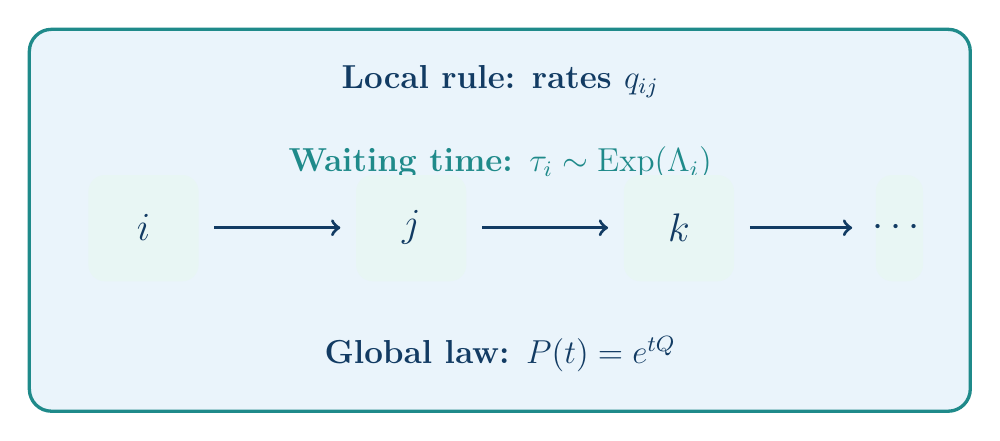
\begin{tikzpicture}[x=1cm,y=1cm]
    \fill[sky,rounded corners=8pt] (0,0) rectangle (11.95,4.85);
    \draw[teal,line width=1.2pt,rounded corners=8pt] (0,0) rectangle (11.95,4.85);
    \node[text=navy,font=\large\bfseries] at (5.98,4.18) {Local rule: rates $q_{ij}$};
    \node[text=teal,font=\large\bfseries] at (5.98,3.15) {Waiting time: $\tau_i\sim\mathrm{Exp}(\Lambda_i)$};
    \node[text=navy,font=\large\bfseries] at (5.98,0.72) {Global law: $P(t)=e^{tQ}$};
    \fill[mint,rounded corners=6pt] (0.75,1.65) rectangle (2.15,3.00);
    \fill[mint,rounded corners=6pt] (4.15,1.65) rectangle (5.55,3.00);
    \fill[mint,rounded corners=6pt] (7.55,1.65) rectangle (8.95,3.00);
    \fill[mint,rounded corners=6pt] (10.75,1.65) rectangle (11.35,3.00);
    \draw[navy,line width=1.2pt,->] (2.35,2.33) -- (3.95,2.33);
    \draw[navy,line width=1.2pt,->] (5.75,2.33) -- (7.35,2.33);
    \draw[navy,line width=1.2pt,->] (9.15,2.33) -- (10.45,2.33);
    \node[text=navy,font=\Large] at (1.45,2.33) {$i$};
    \node[text=navy,font=\Large] at (4.85,2.33) {$j$};
    \node[text=navy,font=\Large] at (8.25,2.33) {$k$};
    \node[text=navy,font=\Large] at (11.05,2.33) {$\cdots$};
  \end{tikzpicture}
  \vspace{0.16cm}

  {\color{navy}\small A unified view of local rates, exponential waiting, and finite-time transition laws.}
\end{frame}

% ---------- Slide 2 ----------
\begin{frame}{Roadmap}
\begin{block}{Main question}
If the process is currently in state $i$, what does the random jump time $\tau_i$ look like, and how does it connect to the generator $Q$ and the finite-time transition matrix $P(t)$?
\end{block}

\vspace{0.18cm}
\begin{columns}[T,totalwidth=\textwidth]
\column{0.485\textwidth}
\begin{alertblock}{Core derivation}
\begin{enumerate}
  \item Local CTMC assumption in a short interval $\Delta t$
  \item Derive the survival function of the first jump time
  \item Read off the density and identify the exponential law
\end{enumerate}
\end{alertblock}

\vspace{0.08cm}
\begin{block}{Takeaway}
The derivation is local, but the conclusion already reveals the full temporal law of the first jump.
\end{block}

\column{0.485\textwidth}
\begin{block}{Unifying interpretations}
\begin{itemize}
  \item survival, density, and hazard
  \item ``when to jump'' vs. ``where to jump''
  \item first-jump decomposition and $P(t)=e^{tQ}$
\end{itemize}
\end{block}

\vspace{0.08cm}
\begin{alertblock}{End goal}
Turn one clean derivation into several equivalent views that reinforce each other.
\end{alertblock}
\end{columns}
\end{frame}

% ---------- Slide 3 ----------
\begin{frame}{Local CTMC assumptions at state $i$}
Assume the process starts from $X_0=i$. For $j\neq i$, define the jump rates
\[
q_{ij}\ge 0,
\qquad
\Lambda_i:=\sum_{j\neq i} q_{ij}.
\]
In a very short interval $\Delta t$,
\[
\Prob(X_{\Delta t}=j\mid X_0=i)=q_{ij}\Delta t+o(\Delta t),\qquad j\neq i,
\]
and therefore the total probability of leaving $i$ is
\[
\Prob(X_{\Delta t}\neq i\mid X_0=i)=\Lambda_i\Delta t+o(\Delta t).
\]
So the probability of \emph{still staying} at $i$ is
\[
\Prob(X_{\Delta t}=i\mid X_0=i)=1-\Lambda_i\Delta t+o(\Delta t).
\]

\begin{alertblock}{Interpretation}
$\Lambda_i$ is the \textbf{total leaving rate}. It controls how fast state $i$ is abandoned; the individual $q_{ij}$ only split that departure into different directions.
\end{alertblock}
\end{frame}

% ---------- Slide 4 ----------
\begin{frame}{Define the waiting time}
The \textbf{waiting time} (or holding time) at state $i$ is the first time the chain leaves $i$:
\[
\tau_i:=\inf\{t>0: X_t\neq i\}.
\]
We want its law.

\vspace{0.2cm}
Define the survival function
\[
S_i(t):=\Prob(\tau_i>t\mid X_0=i).
\]
This means: starting from $i$, the process has \emph{not jumped yet} by time $t$.

\begin{block}{The key recurrence}
To survive until $t+\Delta t$, two things must both happen:
\[
\text{(i) survive until }t,\qquad \text{(ii) then do not leave during }[t,t+\Delta t].
\]
Because of the Markov property, if the chain has not left by time $t$, it is still in state $i$, so the second factor is again
\[
1-\Lambda_i\Delta t+o(\Delta t).
\]
\end{block}
\end{frame}

% ---------- Slide 5 ----------
\begin{frame}{The clean derivation of the exponential law}
Therefore
\[
S_i(t+\Delta t)=S_i(t)\bigl(1-\Lambda_i\Delta t+o(\Delta t)\bigr).
\]
Rearrange:
\[
S_i(t+\Delta t)-S_i(t)=-\Lambda_i S_i(t)\Delta t+o(\Delta t).
\]
Divide by $\Delta t$ and let $\Delta t\to 0$:
\[
S_i'(t)=-\Lambda_i S_i(t),
\qquad
S_i(0)=1.
\]
Hence
\[
S_i(t)=e^{-\Lambda_i t}.
\]
Equivalently,
\[
\Prob(\tau_i>t\mid X_0=i)=e^{-\Lambda_i t}.
\]

\begin{alertblock}{Conclusion}
The waiting time is exponential:
\[
\tau_i\sim \mathrm{Exp}(\Lambda_i).
\]
\end{alertblock}
\end{frame}

% ---------- Slide 6 ----------
\begin{frame}{From survival to density and CDF}
\small
Once we know
\[
\Prob(\tau_i>t)=e^{-\Lambda_i t},
\]
we immediately get the cumulative distribution function
\[
F_{\tau_i}(t)=\Prob(\tau_i\le t)=1-e^{-\Lambda_i t},\qquad t\ge 0.
\]
Differentiate to obtain the density:
\[
f_{\tau_i}(t)=F_{\tau_i}'(t)=\Lambda_i e^{-\Lambda_i t},\qquad t\ge 0.
\]

\begin{columns}[T,totalwidth=\textwidth]
\column{0.52\textwidth}
\begin{block}{Important clarification}
For a continuous random variable,
\[
\Prob(\tau_i=t)=0.
\]
So $f_{\tau_i}(t)$ is \emph{not} the probability of jumping exactly at time $t$.
\end{block}
\column{0.46\textwidth}
\begin{alertblock}{Correct reading}
For small $\Delta t$,
\[
\Prob(t\le \tau_i<t+\Delta t)
\approx f_{\tau_i}(t)\,\Delta t.
\]
It is the probability of the first jump landing in a tiny interval around $t$.
\end{alertblock}
\end{columns}
\end{frame}

% ---------- Slide 7 ----------
\begin{frame}{A very intuitive factorization of the density}
\small
Using the previous slide,
\[
\Prob(t\le \tau_i<t+\Delta t)
\approx \Lambda_i e^{-\Lambda_i t}\Delta t.
\]
This can be read as
\[
\underbrace{e^{-\Lambda_i t}}_{\substack{\text{survive until }t \\\text{(no jump yet)}}}
\times
\underbrace{\Lambda_i\Delta t}_{\substack{\text{jump during the next}\\ \text{tiny interval}}}.
\]
Therefore,
\[
f_{\tau_i}(t)=\underbrace{S_i(t)}_{\text{survival}}\times \underbrace{\Lambda_i}_{\text{hazard}}.
\]

\begin{block}{What changes between these formulas?}
\begin{itemize}
  \item $\Lambda_i\Delta t$ = probability of a jump in the next tiny interval \emph{given that we are still in $i$ now}.
  \item $\Lambda_i e^{-\Lambda_i t}\Delta t$ = probability that the \emph{first} jump lands in $[t,t+\Delta t]$.
\end{itemize}
The extra factor $e^{-\Lambda_i t}$ exactly enforces: \textbf{nothing happened before time $t$}. 
\end{block}
\end{frame}

% ---------- Slide 8 ----------
\begin{frame}{Equivalent interpretations of $\tau_i\sim\mathrm{Exp}(\Lambda_i)$}
\small
\begin{columns}[T,totalwidth=\textwidth]
\column{0.48\textwidth}
\begin{block}{Time scale}
\[
\E[\tau_i]=\frac{1}{\Lambda_i},
\qquad
\mathrm{Var}(\tau_i)=\frac{1}{\Lambda_i^2}.
\]
Large $\Lambda_i$ means short average residence time; small $\Lambda_i$ means the chain tends to stay longer.
\end{block}

\begin{alertblock}{Memoryless property}
\[
\Prob(\tau_i>s+t\mid \tau_i>s)=\Prob(\tau_i>t).
\]
Past waiting does not change the law of future waiting.
\end{alertblock}

\column{0.48\textwidth}
\begin{block}{Hazard interpretation}
\[
\lambda_{\text{haz}}(t)=\frac{f_{\tau_i}(t)}{S_i(t)}=\Lambda_i.
\]
The instantaneous jump intensity is constant as long as the chain is still in state $i$.
\end{block}

\begin{alertblock}{Modeling meaning}
In a neural CTMC or discrete diffusion view, $\Lambda_i$ tells us how quickly the current token/state wants to be rewritten, while the normalized off-diagonal rates decide \emph{where} it jumps.
\end{alertblock}
\end{columns}
\end{frame}

% ---------- Slide 9 ----------
\begin{frame}{``When to jump'' and ``where to jump'' are different objects}
Suppose the chain is currently in state $i$.
\[
\Lambda_i=\sum_{j\neq i} q_{ij}.
\]
Then the CTMC jump mechanism splits neatly into two parts:

\begin{block}{1. When to jump}
\[
\tau_i\sim \mathrm{Exp}(\Lambda_i).
\]
Only the \textbf{sum} of outgoing rates matters.
\end{block}

\begin{alertblock}{2. Where to jump}
Conditioned on a jump occurring, the destination is
\[
\Prob(X_{\tau_i}=j\mid X_0=i,\text{ a jump occurs})=\frac{q_{ij}}{\Lambda_i},\qquad j\neq i.
\]
Only the \textbf{relative proportions} of the off-diagonal rates matter.
\end{alertblock}

\vspace{0.06cm}
This is the fundamental decomposition:
\[
\textbf{local speed} \quad \Longleftrightarrow \quad \Lambda_i,
\qquad
\textbf{jump direction} \quad \Longleftrightarrow \quad \frac{q_{ij}}{\Lambda_i}.
\]
\end{frame}

% ---------- Slide 10 ----------
\begin{frame}{Generator form and the short-time transition matrix}
\small
Define the generator by
\[
q_{ii}:=-\sum_{j\neq i}q_{ij}=-\Lambda_i.
\]
Then every row sums to zero:
\[
\sum_j q_{ij}=0.
\]
The short-time transition matrix satisfies
\[
P(\Delta t)=I+\Delta t\,Q+o(\Delta t).
\]
In components,
\[
P_{ij}(\Delta t)\approx q_{ij}\Delta t\quad (j\neq i),
\qquad
P_{ii}(\Delta t)\approx 1-\Lambda_i\Delta t.
\]

\begin{block}{Probability conservation}
The row-sum-zero condition is exactly what makes each row of $P(\Delta t)$ sum to $1$ to first order:
\[
\sum_j P_{ij}(\Delta t)\approx 1+\Delta t\sum_j q_{ij}=1.
\]
\end{block}
\end{frame}

% ---------- Slide 11 ----------
\begin{frame}{Do not confuse $\Prob(\tau_i>t)$ with $P_{ii}(t)$}
\small
These two quantities are closely related but generally \textbf{not equal}:
\[
\Prob(\tau_i>t\mid X_0=i)=e^{-\Lambda_i t}
\]
and
\[
P_{ii}(t)=\Prob(X_t=i\mid X_0=i).
\]

\begin{columns}[T,totalwidth=\textwidth]
\column{0.49\textwidth}
\begin{block}{What $\Prob(\tau_i>t)$ means}
The process has \textbf{never left} state $i$ during the whole interval $[0,t]$.
\end{block}
\column{0.49\textwidth}
\begin{alertblock}{What $P_{ii}(t)$ means}
At time $t$, the process is in $i$ again. It may have left earlier and then returned.
\end{alertblock}
\end{columns}

\vspace{0.12cm}
Therefore, usually
\[
\Prob(\tau_i>t\mid X_0=i)\le P_{ii}(t).
\]
The first quantity is about the \textbf{first jump time}; the second is about the \textbf{full law at time $t$}.
\end{frame}

% ---------- Slide 12 ----------
\begin{frame}{First-jump decomposition: the bridge to finite-time laws}
\small
Starting from $i$, to be in state $j$ at time $t$, we can condition on the first jump time.

For $j\neq i$,
\[
P_{ij}(t)=\sum_{k\neq i}\int_0^t e^{-\Lambda_i s}\,q_{ik}\,P_{kj}(t-s)\,\dd s.
\]
For $j=i$,
\[
P_{ii}(t)=e^{-\Lambda_i t}+\sum_{k\neq i}\int_0^t e^{-\Lambda_i s}\,q_{ik}\,P_{ki}(t-s)\,\dd s.
\]

\begin{block}{How to read it}
\begin{itemize}
  \item $e^{-\Lambda_i s}$: no jump before time $s$
  \item $q_{ik}\,\dd s$: first jump occurs in $[s,s+\dd s]$ and lands in $k$
  \item $P_{kj}(t-s)$: evolve from $k$ for the remaining time
\end{itemize}
\end{block}

This decomposition is the cleanest way to see how the exponential waiting law feeds into the full finite-time transition matrix.
\end{frame}

% ---------- Slide 13 ----------
\begin{frame}{From the semigroup property to the ODE for $P(t)$}
\small
The finite-time transition matrix satisfies the semigroup property
\[
P(t+s)=P(t)P(s),
\qquad P(0)=I.
\]
Set $s=\Delta t$. Then
\[
P(t+\Delta t)=P(t)P(\Delta t).
\]
Using the short-time expansion
\[
P(\Delta t)=I+\Delta tQ+o(\Delta t),
\]
we obtain
\[
P(t+\Delta t)=P(t)\bigl(I+\Delta tQ+o(\Delta t)\bigr)
= P(t)+\Delta t\,P(t)Q+o(\Delta t).
\]
Therefore
\[
\frac{P(t+\Delta t)-P(t)}{\Delta t}=P(t)Q+o(1),
\]
and letting $\Delta t\to 0$ gives
\[
P'(t)=P(t)Q,
\qquad P(0)=I.
\]

\begin{block}{Interpretation}
The local generator $Q$ controls the instantaneous change of the whole transition matrix. The exponential waiting law is the one-state shadow of this global evolution equation.
\end{block}
\end{frame}

% ---------- Slide 14 ----------
\begin{frame}{Why the solution is the matrix exponential}
\small
We now solve
\[
P'(t)=P(t)Q,
\qquad P(0)=I.
\]
Define the matrix exponential by the power series
\[
e^{tQ}:=\sum_{n=0}^{\infty}\frac{(tQ)^n}{n!}
=I+tQ+\frac{t^2Q^2}{2!}+\cdots.
\]
Differentiate term by term:
\[
\frac{\dd}{\dd t}e^{tQ}
=\sum_{n=1}^{\infty}\frac{n t^{n-1}Q^n}{n!}
=\sum_{m=0}^{\infty}\frac{t^mQ^{m+1}}{m!}
=e^{tQ}Q.
\]
Also,
\[
e^{0\cdot Q}=I.
\]
Hence $e^{tQ}$ satisfies exactly the same ODE and initial condition, so
\[
\boxed{P(t)=e^{tQ}}.
\]

\begin{alertblock}{Equivalent discrete-time intuition}
If $t=n\Delta t$, then $P(t)=P(\Delta t)^n\approx \left(I+\frac{t}{n}Q\right)^n \to e^{tQ}$.
\end{alertblock}
\end{frame}

% ---------- Slide 15 ----------
\begin{frame}{Why every row of $P(t)$ sums to $1$}
\small
Because
\[
q_{ii}=-\sum_{j\neq i}q_{ij},
\]
we have row-sum zero for the generator:
\[
\sum_j q_{ij}=0.
\]
In vector form, with $\mathbf 1=(1,\dots,1)^\top$,
\[
Q\mathbf 1=0.
\]
Now use the matrix exponential representation:
\[
P(t)\mathbf 1=e^{tQ}\mathbf 1
=\left(I+tQ+\frac{t^2Q^2}{2!}+\cdots\right)\mathbf 1.
\]
Since $Q\mathbf 1=0$, all higher terms vanish as well:
\[
Q^2\mathbf 1=Q(Q\mathbf 1)=0,
\qquad Q^3\mathbf 1=0,
\qquad \cdots
\]
Therefore
\[
P(t)\mathbf 1=\mathbf 1.
\]
So each row of $P(t)$ sums to $1$, exactly as a transition probability matrix should.

\begin{block}{Big picture}
The condition $Q\mathbf 1=0$ is the infinitesimal form of probability conservation; the identity $P(t)\mathbf 1=\mathbf 1$ is the finite-time form.
\end{block}
\end{frame}

% ---------- Slide 16 ----------
\begin{frame}{A two-state example that separates the concepts}
\small
Consider
\[
Q=
\begin{pmatrix}
-a & a\\
 b & -b
\end{pmatrix}.
\]
Starting from state $0$, the total leaving rate is $\Lambda_0=a$, so
\[
\tau_0\sim \mathrm{Exp}(a),
\qquad
\Prob(\tau_0>t)=e^{-at}.
\]
But the finite-time probability of being in state $0$ is
\[
P_{00}(t)=\frac{b}{a+b}+\frac{a}{a+b}e^{-(a+b)t}.
\]

\begin{columns}[T,totalwidth=\textwidth]
\column{0.49\textwidth}
\begin{block}{First quantity}
$e^{-at}$ means: \emph{never left state 0 up to time $t$}.
\end{block}
\column{0.49\textwidth}
\begin{alertblock}{Second quantity}
$P_{00}(t)$ means: \emph{is in state 0 at time $t$}, possibly after leaving and returning.
\end{alertblock}
\end{columns}

This example is often the fastest way to remove the main conceptual confusion.
\end{frame}

% ---------- Slide 17 ----------
\begin{frame}{Takeaways}
\small
\begin{block}{Core facts}
\begin{enumerate}
  \item At state $i$, the total leaving rate is $\Lambda_i=\sum_{j\neq i}q_{ij}$.
  \item The waiting time is exponential:
  \[
  \tau_i\sim \mathrm{Exp}(\Lambda_i).
  \]
  \item The density is
  \[
  f_{\tau_i}(t)=\Lambda_i e^{-\Lambda_i t}=S_i(t)\times \Lambda_i.
  \]
\end{enumerate}
\end{block}

\begin{alertblock}{The big picture}
\textbf{When to jump} is governed by the exponential waiting law. \textbf{Where to jump} is governed by the normalized off-diagonal rates. Putting all local moves together gives the finite-time law
\[
P(t)=e^{tQ}.
\]
\end{alertblock}
\end{frame}

\end{document}
